\documentclass[11pt, a4paper, oneside]{article}

\usepackage[utf8]{inputenc}
\usepackage[margin=0.8in]{geometry}
\usepackage{amsmath,amssymb,amsfonts,amsthm}
\usepackage{graphics}
\usepackage[export]{adjustbox}
\usepackage{wrapfig}
\usepackage{hyperref}
\usepackage{cite}
\usepackage{ebgaramond}
\usepackage[defaultsans]{lato}
\usepackage{enumerate}
\usepackage{fancyhdr}
\usepackage{array}
\usepackage{etoolbox}

\pagestyle{fancyplain}

\fancyhf{} % sets both header and footer to nothing
\renewcommand{\headrulewidth}{0pt}
\fancyhead[L]{}% Empty left header
\fancyhead[C]{} % Page numbering for center header  
\fancyhead[R]{}% Empty right header
\fancyfoot[L]{}% Empty left footer
\fancyfoot[C]{\thepage}% Empty center footer
\fancyfoot[R]{}% Empty left footer

\patchcmd{\thebibliography}{\section*{\refname}}{}{}{}

\newcolumntype{L}[1]{>{\raggedright\let\newline\\\arraybackslash\hspace{0pt}}m{#1}}
\newcolumntype{C}[1]{>{\centering\let\newline\\\arraybackslash\hspace{0pt}}m{#1}}
\newcolumntype{R}[1]{>{\raggedleft\let\newline\\\arraybackslash\hspace{0pt}}m{#1}}

\begin{document}

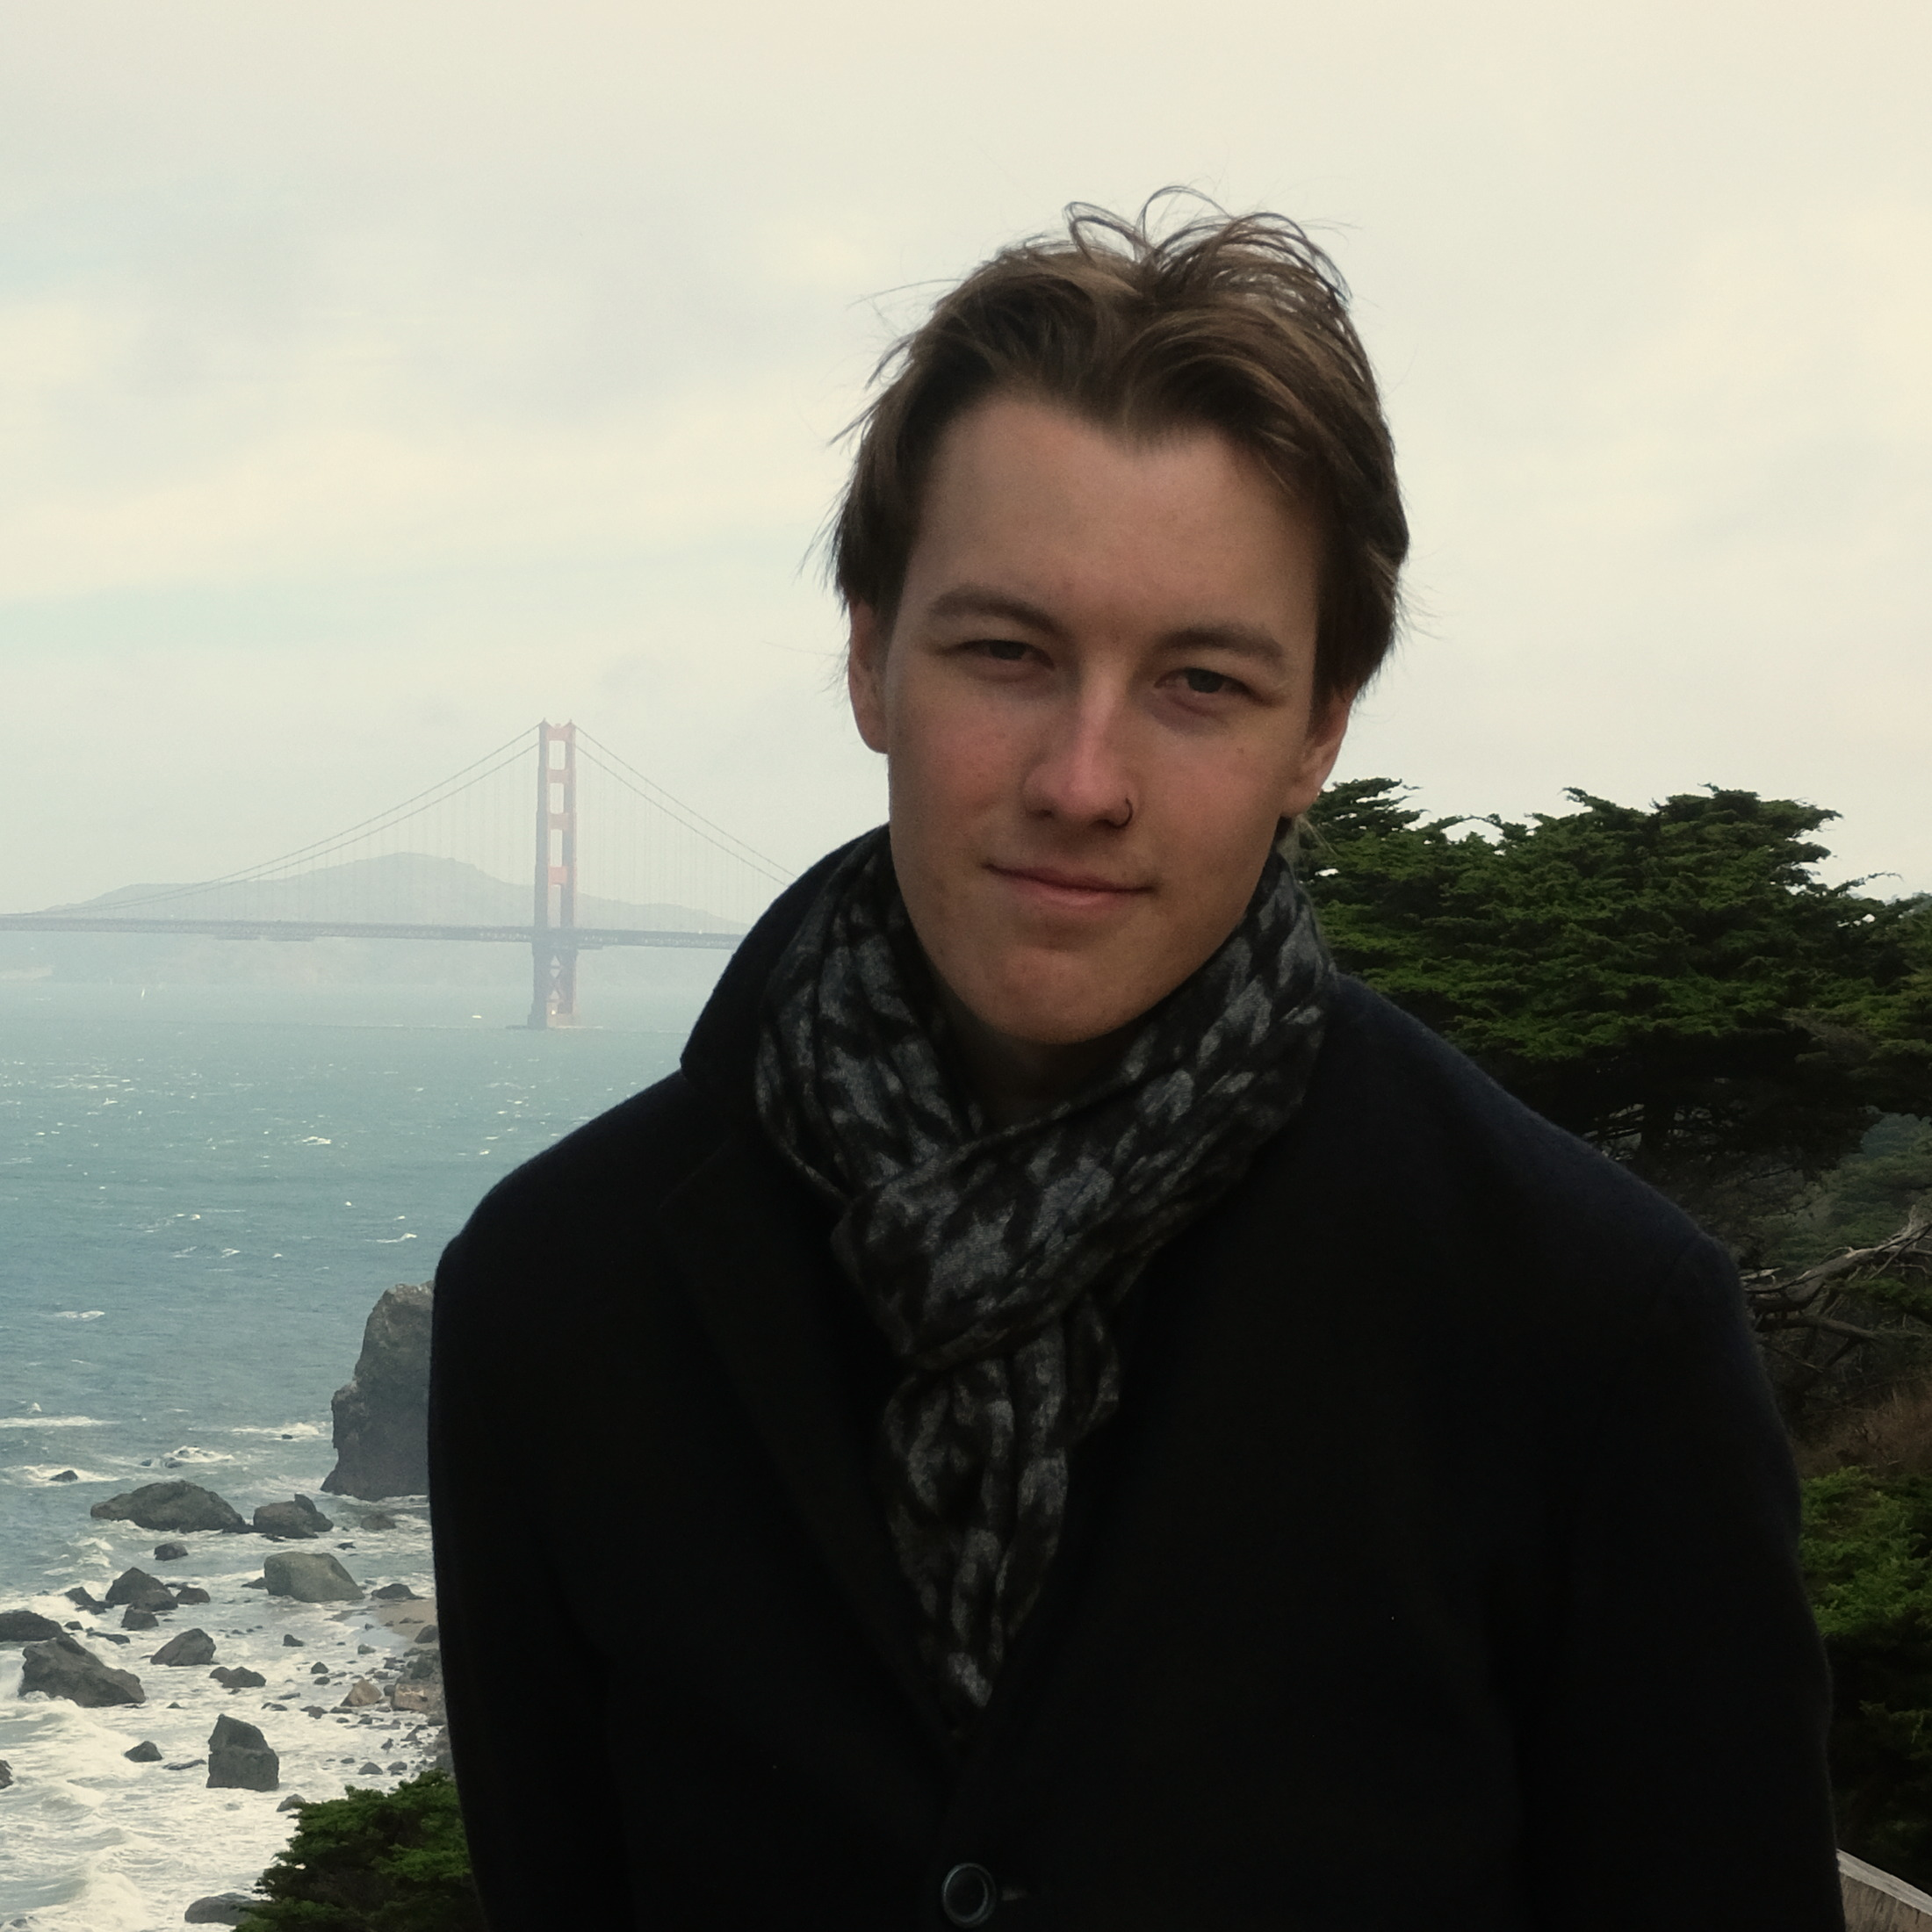
\includegraphics[width=0.3\linewidth, right]{Tassilo} 
\vspace*{-15em}
\begin{flushleft}
\hspace*{1.3em} \huge Tassilo Tanneberger
\vspace*{-0.5em}
\par\noindent\rule{0.6\textwidth}{0.4pt}
\end{flushleft}

\vspace*{-0.4em}

\begin{tabular}{l}
TUD Dresden University of Technology  \\
Faculty of Computer Science \\ 
Chair of Compiler Construction \\ 
\href{mailto: tassilo.tanneberger@tu-dresden.de}{\texttt{tassilo.tanneberger@tu-dresden.de}} \\
\href{https://tanneberger.me}{\texttt{https://tanneberger.me}} \\
\href{https://github.com/tanneberger}{\texttt{https://github.com/tanneberger}}
\end{tabular}

\par\noindent\rule{0.6\textwidth}{0.4pt}

\section*{Research Interests}

Domain Specific Languages (DSLs), Distributed Systems, Embedded Systems, Scheduling Theory, \\ RTOS,  Deterministic Concurrency.  

\section*{Education}

\begin{tabular}{ R{3cm} L{10cm}}
	2021 - 2026 &  Study of Computer Science (Diploma) \\
							& TUD Dresden University of Technology \\ 
							&			\\
	5/2021			& Grammerschool with Grade 1.7
\end{tabular}


\section*{Professional Experience}

\begin{tabular}{R{3cm} L{12cm}}
	2023 	- now				& Co-founder and Member of Board of Directors \\ & DD-IX Dresden Internet Exchange e.V. \\ & \\
	11/2021 	- now			& Research Student at the Chair for Compiler Construction, \\ 
										& TUD Dresden University of Technology \\ 
										& 																			\\
	4/2021 - 10/2021    & Engineer working on Tooling for Industrial Robots \\ 
										& Society for the Advancement of Applied Computer Science (GFaI)
\end{tabular}


\section*{Open Source Projects}

\begin{tabular}{R{3cm} L{13cm}}
	2022 							    & TLMS - Transit Live Mapping Solutions \\
	  										&	\emph{Reverse engineering of the radio protocol used for controlling traffic lights in Germany. Design and implementation of a platform that shows live positions of trams and buses based on this data.} \href{https://map.tlm.solutions}{\texttt{https://tlm.solutions}}  \\  
	  										& \\
		2021 							& Lingua-Franca (LF) - a polyglot coordination language for reactive, concurrent, and time-sensitive applications.  \\ 
											& \emph{Optimization of the C++ runtime environment, development  of  a package manager and built tool for the LF ecosystem.} \href{https://lf-lang.org}{\texttt{https://lf-lang.org}} \\
\end{tabular}

\section*{Extracurricular Activities}

\begin{tabular}{R{3cm} L{13cm}}
	11/2023 - now   	& Task-Force for the Strategic Development of the Faculty \\ 
									& Faculty of Computer Science, TUD Dresden University of Technology  \\ & \\
	11/2022 - now 	    & Member of the Faculty Council \\ 
									& Faculty of Computer Science, TUD Dresden University of Technology 
\end{tabular}


\section*{Publications}

\nocite{*} 
\bibliographystyle{ACM-Reference-Format}
\bibliography{refs}{}

\end{document}
